\subsection{平面}\label{subsec:1-1}

常见的桌面、黑板面、平静的水面以及纸板等,都给我们以平面的形象。几何里所说的平面
就是从这样的一些物体抽象出来的。但是,几何里的平面是无限延展的。

当我们从适当的角度和距离观察桌面或黑板面时,感到它们都很象平行四边形。因此,在
立体几何中,通常画平行四边形来表示平面(图 \ref{fig:ltjh-1-1})。当平面是水平放置的时候,通常把
平行四边形的锐角画成 $45^\circ$,横边画成等于邻边的两倍。当一个平面的一部分被
另一个平面遮住时,应把被遮部分的线段画成虚线或不画(图 \ref{fig:ltjh-1-2})。这样,看起来立体感强一些。

\begin{figure}[htbp]
    \centering
    \begin{minipage}[b]{7cm}
        \centering
        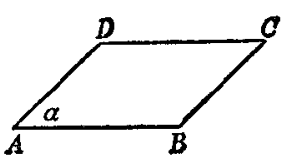
\includegraphics[width=4cm]{../pic/ltjh-ch1-01.png}
        \caption{}\label{fig:ltjh-1-1}
    \end{minipage}
    \qquad
    \begin{minipage}[b]{7cm}
        \centering
        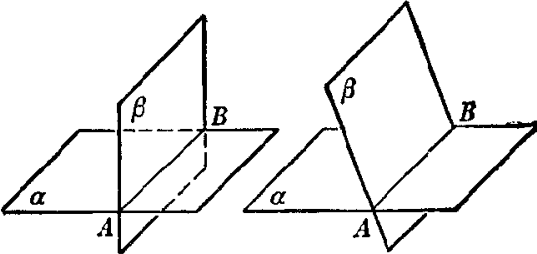
\includegraphics[width=7cm]{../pic/ltjh-ch1-02.png}
        \caption{}\label{fig:ltjh-1-2}
    \end{minipage}
\end{figure}

平面通常用一个希腊字母 $\alpha$、$\beta$、$\gamma$ 等来表示,如平面 $\alpha$、
平面 $\beta$、平面 $\gamma$ 等,也可以用表示平行四边形的两个相对顶点的字母来表示,
如平面 $AC$ (图 \ref{fig:ltjh-1-1})。


\begin{lianxi}

\xiaoti{能不能说一个平面长 $4$ 米,宽 $2$ 米?为什么?}

\xiaoti{观察 (1)、(2) 中甲、乙两个图形,用模型来说明它们的位置有什么不同。
    并用字母来表示各平面。
}

\begin{figure}[htbp]
    \centering
    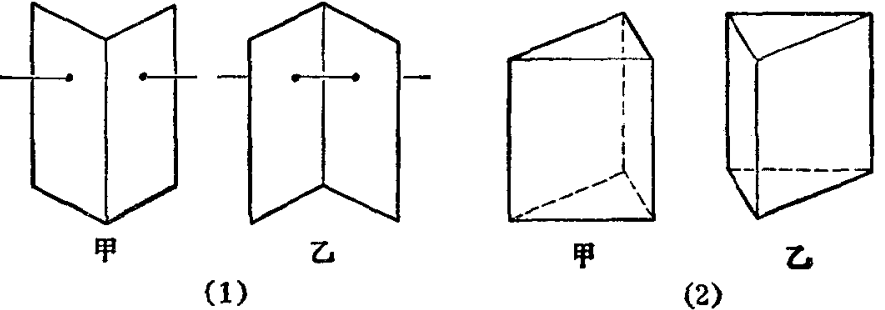
\includegraphics[width=10cm]{../pic/ltjh-ch1-subsec1-lx-02.png}
    \caption*{(第 2 题)}
\end{figure}

\end{lianxi}

